% Тут используется класс, установленный на сервере Papeeria. На случай, если
% текст понадобится редактировать где-то в другом месте, рядом лежит файл matmex-diploma-custom.cls
% который в момент своего создания был идентичен классу, установленному на сервере.
% Для того, чтобы им воспользоваться, замените matmex-diploma на matmex-diploma-custom
% Если вы работаете исключительно в Papeeria то мы настоятельно рекомендуем пользоваться
% классом matmex-diploma, поскольку он будет автоматически обновляться по мере внесения корректив
%

% По умолчанию используется шрифт 14 размера. Если нужен 12-й шрифт, уберите опцию [14pt]
\documentclass[14pt]{matmex-diploma}
%\documentclass[14pt]{matmex-diploma-custom}

\begin{document}
% Год, город, название университета и факультета предопределены,
% но можно и поменять.
% Если англоязычная титульная страница не нужна, то ее можно просто удалить.
\filltitle{ru}{
    chair              = {Кафедра Системного программирования},
    title              = {Разработка архитектуры для унификации синтаксических анализаторов в проекте YaccConstructor},
    % Здесь указывается тип работы. Возможные значения:
    %   coursework - Курсовая работа
    %   diploma - Диплом специалиста
    %   master - Диплом магистра
    %   bachelor - Диплом бакалавра
    type               = {coursework},
    position           = {студента},
    group              = 344,
    author             = {Соловьев Александр Александрович},
    supervisorPosition = {ст. преп., к.\,ф.-м.\,н.},
    supervisor         = {Григорьев С.\,В.}
}
\maketitle
\tableofcontents

\section*{Введение}
В области синтаксического анализа существует множество различных задач. Наиболее известной из них является задача анализа некоторой последовательности токенов с целью проверки ее выводимости в заданной грамматике и построением соответствующего дерева вывода. Однако данная задача может быть рассмотрена более широко, поскольку подвергаться синтаксическому анализу могут не только строки, но и другие структуры данных. Например, в работах \cite{graphParseVerb} и \cite{graphParseRag} в качестве объекта синтаксического анализа рассматривается граф.

В 2010 году был предложен алгоритм обобщенного анализа Generalized LL(GLL), в основе которого лежит алгоритм нисходящего синтаксического анализа~\cite{GLLParsing}. Данный алгоритм и различные его модификации были реализованы в проекте YaccConstructor~\cite{YaccConstructor} независимо друг от друга. Различия их заключаются в первую очередь в структурах данных, которые подаются на вход, а также в возможности построения с помощью этих алгоритмов деревьев вывода. Конечно, отличается также и их внутренняя реализация, но общая структура различных версий при этом не меняется. Из сказанного выше следует, что поддерживать и сопровождать приходится все реализованные алгоритмы. Эту проблему могло бы решить их обобщение. Теоретически оно возможно, однако на практике возможно возникновение различных трудностей, получившееся решение может обладать рядом недостатков по сравнению с набором отдельно реализованных алгоритмов. Например, решение может быть крайне громоздким, что может еще больше усложнить его поддержку, одним же из наиболее вероятных недостатков, которые могут возникнуть, является значительное падение производительности. Например, при попытке представить линейный вход в виде графа, появляются циклы для перебора всех исходящих из вершины ребер, что приводит к увеличению числа операций.

\section{Постановка задачи}
Целью данной работы является разработка архитектуры для унификации существующих синтаксических анализаторов в проекте \newline YaccConstructor. Для достижения данной цели были поставлены следующие задачи:
\begin{itemize}
    \item спроектировать архитектуру, позволяющую объединить различные модификации алгоритма;
    \item реализовать предложенную архитектуру;
    \item разработать тестовое покрытие;
    \item провести эксперименты для оценки производительности.
\end{itemize}

\section{Обзор}
\subsection{YaccConstructor}
YaccConstructor --- проект, разрабатываемый в лаборатории языковых инструментов JetBrains, расположенной на кафедре системного программирования. В нем занимаются исследованиями и разработками в области лексического и синтаксического анализа. Большинство компонентов проекта реализованы на языке F\#, исходный код проекта находится в открытом доступе \cite{YaccConstructor}. Проект имеет модульную архитектуру (рис.\ref{fig:YCArch}), что позволяет собирать требуемый инструмент из существующих модулей: можно выбрать фронтенд, задать требуемые преобразования грамматики и указать генератор. Генераторы предоставляют инструменты, позволяющие по внутреннему представлению грамматики получить полезный для конечного пользователя результат. Примером такого результата являются синтаксические анализаторы.

\begin{figure}[h]
	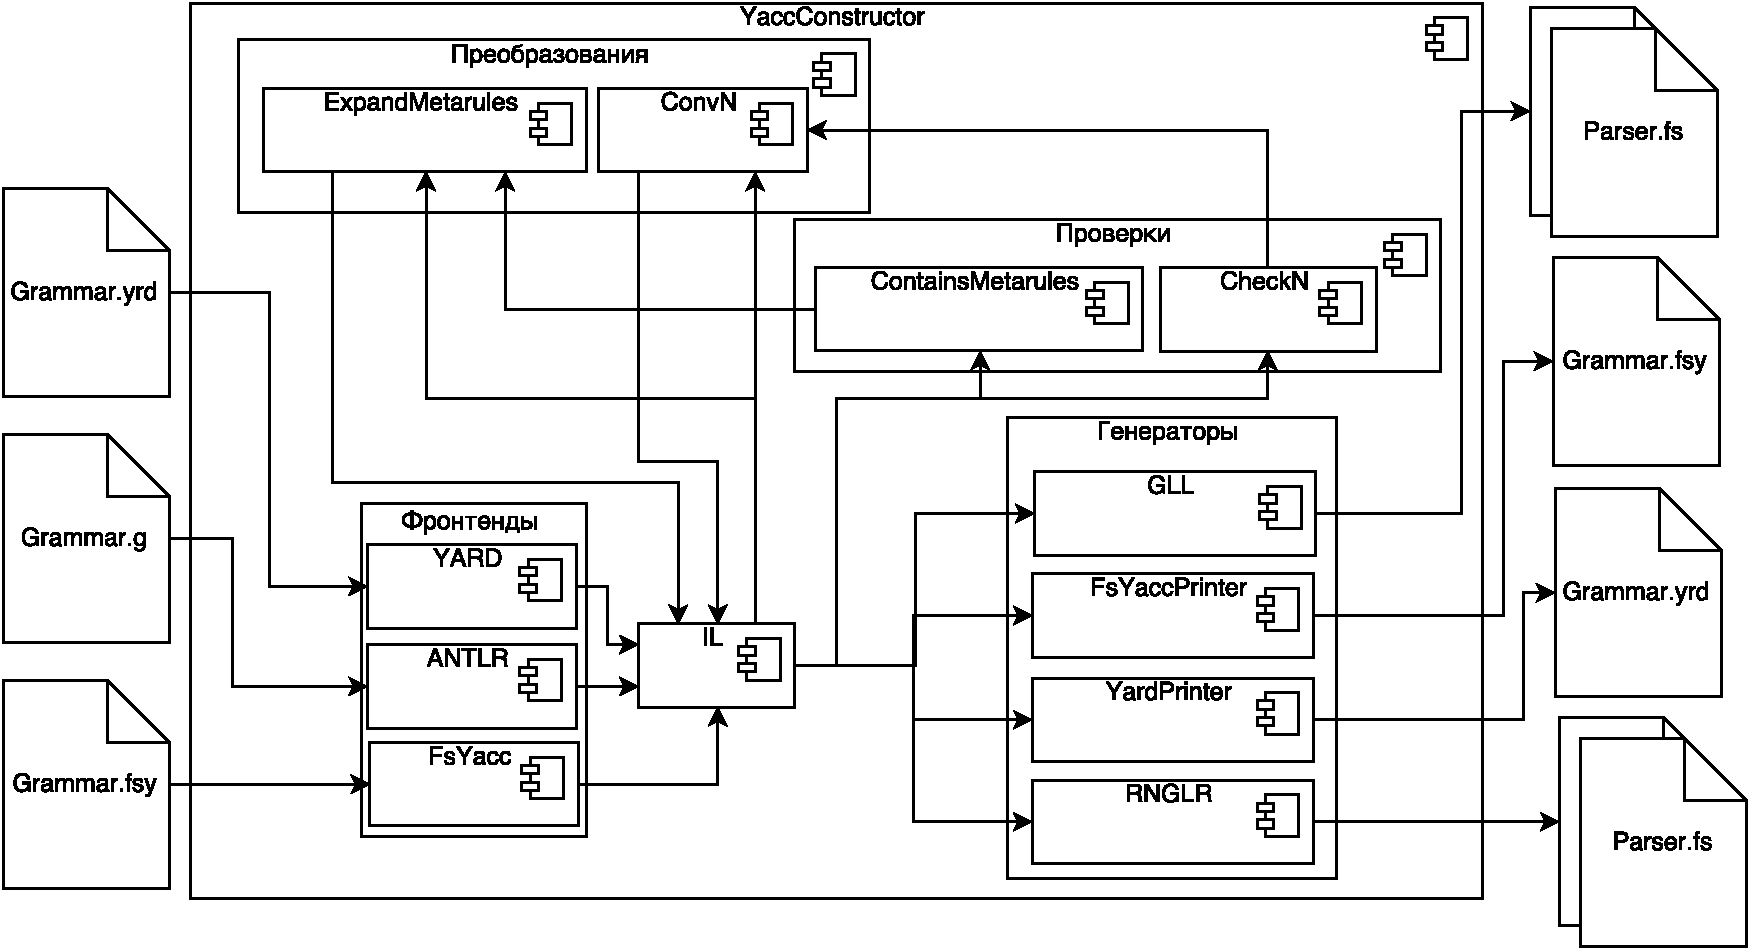
\includegraphics[width=\textwidth]{images/YCArch}
	\caption{Архитектура YaccConstructor, заимствована из \cite{gsvPhd}}
	\label{fig:YCArch}
\end{figure}

\subsection{Синтаксические анализаторы, основанные на GLL}
Как говорилось выше, на данный момент в проекте реализованы GLL и несколько его модификаций. Различаются они в рассматриваемой структуре данных, в возможности построения дерева вывода, а также в том, подается ли на вход алгоритму грамматика или же рекурсивный автомат \cite{RADesc}. 

Далеее перечислены модификации алгоритма, которые на данный момент реализованы в YaccConstructor. Все перечисленные, помимо последней, версии умеют строить деревья вывода:
\begin{itemize}
    \item стандартная версия алгоритма, принимающая на вход грамматику и последовательность токенов;
    \item алгоритм, принимающий на вход грамматику и граф ;
    \item алгоритм, принимающий на вход грамматику и GFG \cite{GFGDesc};
    \item алгоритм, принимающий на вход конечный автомат и последовательность токенов;
    \item алгоритм, принимающий на вход конечный автомат и граф.
\end{itemize}

\section{Заключение}
Достигнуты следующие результаты:
\begin{itemize}
    \item произведен обзор статей, связанных с предметной областью;
    \item спроектирована архитектура;
\end{itemize}
В дальнейшем планируется:
\begin{itemize}
    \item реализовать предложенную архитектуру;
    \item разработать тестовое покрытие;
    \item провести эксперименты для оценки производительности.
\end{itemize}


\setmonofont[Mapping=tex-text]{CMU Typewriter Text}
\bibliographystyle{ugost2008ls}
\bibliography{diploma.bib}
\end{document}
